\documentclass[openary, a4paper, oneside]{jsarticle}

\input{../../mymacro.tex}

\newcommand{\Dt}{\frac{d}{dt}}
\newcommand{\Ds}{\frac{d}{ds}}
\newcommand{\dt}{\partial_t}
\newcommand{\ds}{\partial_s}
\newcommand{\dnu}{\partial_{\nu}}

\newcommand{\sG}{_{\Gamma}}
\newcommand{\sS}{_{\Sigma}}

\newcommand{\veps}{\varepsilon}

\newcommand{\INTt}{\int_0^t}
\newcommand{\INTT}{\int_0^T}
\newcommand{\INTO}{\int_{\Omega}}
\newcommand{\INTG}{\int_{\Gamma}}

\newcommand{\weakto}{\rightharpoonup}
\newcommand{\weakstarto}{\overset{*}{\rightharpoonup}}
\newcommand{\emb}{\hookrightarrow}
\newcommand{\emp}{\hookleftarrow}

\newcommand{\Otani}{\^Otani}
\newcommand{\Holder}{H\"older}
\newcommand{\Schrodinger}{Schr\"odinger}
\newcommand{\Arzela}{Arzel\`a}
\newcommand{\Poincare}{Poincar\'e}
\newcommand{\Komura}{K\=omura}

\usepackage{tikz}
\usetikzlibrary{positioning}

\renewcommand{\thethm}{\arabic{section}.\arabic{thm}}
\author{香川 渓一郎}
\date{\today}
\title{Cahn--Hilliard equation 関連論文}
\hypersetup{
	pdfkeywords={},
	pdfsubject={},
	pdfcreator={}
}

\renewcommand{\labelenumi}{(\arabic{enumi})}

\begin{document}

\maketitle
\tableofcontents

\section{Cahn-Hilliard equation}
引用被引用関係を有向グラフにまとめる.

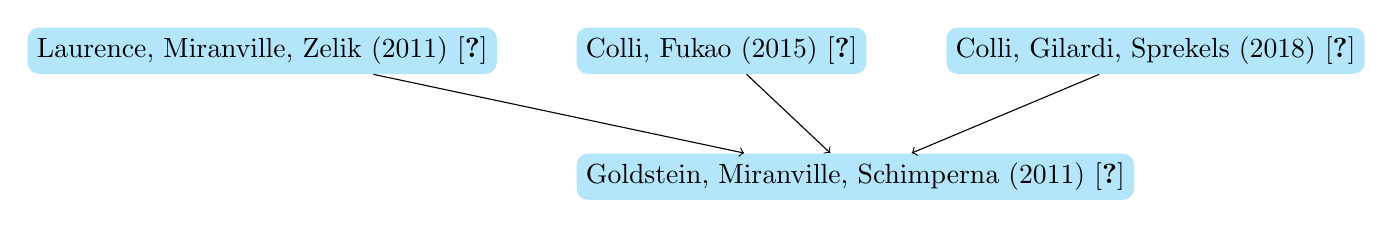
\begin{tikzpicture}[every node/.style={rectangle,fill=cyan!30,rounded corners}]
    \node (GMS) {Goldstein, Miranville, Schimperna (2011) \cite{GoldsteinMiranvilleSchimperna2011}};
    \node[above left=of GMS] (LMS) {Laurence, Miranville, Zelik (2011) \cite{LaurenceMiranvilleZelik2011}};
    \node[right=of LMS] (CF) {Colli, Fukao (2015) \cite{ColliFukao2015}};
		\node[right=of CF] (CGS) {Colli, Gilardi, Sprekels (2018) \cite{ColliGilardiSprekels2018}};

    \foreach \u / \v in {LMS/GMS,CF/GMS,CGS/GMS}
        \draw[->] (\u) -- (\v);
\end{tikzpicture}

\begin{thebibliography}{99}
	\bibitem{GoldsteinMiranvilleSchimperna2011}
	Goldstein, Gis\`ele Ruiz, Alain Miranville, and Giulio Schimperna. "A Cahn–Hilliard model in a domain with non-permeable walls." Physica D: Nonlinear Phenomena 240.8 (2011): 754-766.
	\bibitem{LaurenceMiranvilleZelik2011}
	Cherfils, Laurence, Alain Miranville, and Sergey Zelik. "The Cahn-Hilliard equation with logarithmic potentials." Milan Journal of Mathematics 79.2 (2011): 561-596.
	\bibitem{ColliFukao2015}
	Colli, Pierluigi, and Takeshi Fukao. "Equation and dynamic boundary condition of Cahn--Hilliard type with singular potentials." Nonlinear Analysis: Theory, Methods \& Applications 127 (2015): 413-433.
	\bibitem{ColliGilardiSprekels2018}
	Colli, Pierluigi, Gianni Gilardi, and J\"urgen Sprekels. "On a Cahn–Hilliard system with convection and dynamic boundary conditions." Annali di Matematica Pura ed Applicata (1923-) 197.5 (2018): 1445-1475.
\end{thebibliography}

\end{document}
